\chapter{Continuo  monodimensionale}

\section{Introduzione}


In questo capitolo ci occuperemo di descrivere la cinematica di corpi monodimensionali. Il vantaggio di anteporre ad una generica trattazione in tre dimensioni l'analisi di corpi monodimensionali consiste innanzitutto di ridurre al minimo la complessità analitica, pur restando sufficientemente rappresentativa degli elementi essenziali che si incontreranno nel capitolo successivo.





\section{Deformazione}

Un \textit{corpo}  $\mathcal{B}$ è una varietà di \textit{punti materiali}, che denotiamo con $X$. Assumiamo che questi punti siano elementi primitivi della Meccanica, esattamente come i numeri lo sono in Analisi.


Supporremo che i corpi siano in grado di occupare varie  regioni dello spazio ambiente, che in questo capitolo identificheremo con lo spazio Euclideo monodimensionale $\Ec^{(1)}$; naturalmente associato ad $\Ec^{(1)}$ è lo spazio vettoriale delle traslazioni, che qui indichiamo con $\Vc^{(1)}$. Indicheremo con $\eb$ il vettore unitario che orienta lo spazio, sicché ogni vettore $\vb$ di $\Vc^{(1)}$ non sarà altro che un multiplo di $\eb$: $\vb =v\eb$, $v\in \Ro$.

Nella meccanica dei continui, la varietà $\Bc$ è generalmente assunta regolare, ovvero un diffeormorfismo di un dominio nello spazio Euclideo. In questo primo modello che sviluppiamo, supponiamo che tanto $\Bc$ che lo spazio Euclideo siano monodimensionali.

Affermiamo che un insieme aperto $\Omega$ nello spazio $\Ec^{(1)}$ è occupato dal corpo $\Bc$ qualora esista una funzione \textit{iniettiva}, denominata \textit{piazzamento} o \textit{configurazione}, che mappa $\Bc$ in $\Omega$:
\begin{equation}
\kappa\,:\,\Bc\to \Omega\in \Ec^{(1)}.
\end{equation}
Il piazzamento $\kappa$ mappa dunque i punti materiali $X$ in punti $x$ dello spazio Euclideo; $\xb \coloneqq x\eb$ è dunque la posizione occupata dal punto $X$ nel piazzamento $\kappa$. 


\begin{center}
		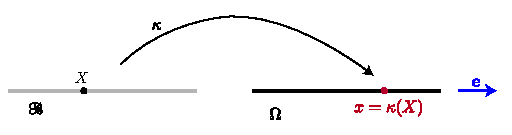
\includegraphics[scale=1.3]{figure/cinematica/piazzamento1d}
\end{center}


L’iniettività dei piazzamenti  assicura che ad ogni punto dello spazio Euclideo corrisponda al più un singolo punto materiale. Tale assunzione evita la ``compenetrazione della materia''. Inoltre, supporremo che i piazzamenti siano \textit{suriettivi}, ovvero che per ogni punto $\Bc$ nell'insieme $\Omega$, esista almeno un punto $\kappa(\Bc)$: in altri termini, il piazzamento non crea nuovi punti.

Ne segue che il piazzamento $\kappa$ è una mappa \textit{biiettiva} e dunque ammette un'inversa
\begin{equation}
	\kappa^{-1}\,:\,\kappa(\Bc)=\Omega\mapsto\Bc.
\end{equation}

Se $\chi$ è un altro piazzamento, possiamo definire la funzione
\begin{equation}
	f \,:\, \kappa(\Bc)\mapsto\chi(\Bc)
\end{equation}
come $f\coloneqq\chi\circ \kappa^{-1}$. Tale funzione è la \textit{deformazione}\footnote{Qualche trattatista chiama questa funzione \textit{trasporto}, piuttosto che deformazione, per distinguere quelle $f$ che inducono cambiamenti di geometria che producono variazioni \textit{metriche}, di lunghezze, aree, angoli  (che chiamano appunto deformazioni) da quelle che non lo fanno, come le traslazioni e le rotazioni. Noi preferiremo la denominazione \textit{deformazione}, alludendo ad un generico cambiamento della configurazione geometrica del corpo, come suggerisce l'etimologia. } dalla configurazione $\kappa$ alla configurazione $\chi$. Dunque, se $\xb\equiv x \,\eb=\kappa(X)$, diremo che $\xb$ e $f(x)\eb$ sono rispettivamente le posizioni occupate dal punto materiale $X$ prima e dopo la deformazione $f$.

\begin{center}
	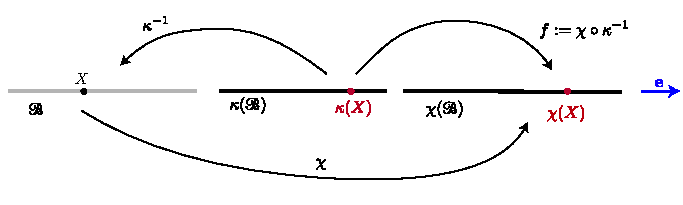
\includegraphics[scale=1.3]{figure/cinematica/def1d}
\end{center}

Assumiamo  che la mappa di deformazione $f$ sia continua e differenziabile, il che evita situazioni patologiche come la frattura, che in questo corso non considereremo.

\subsection{Gradiente della deformazione}
Data una deformazione $f(x)$, il gradiente della deformazione si introduce per `esplorare' cosa accade in un intorno di $x$, muovendosi nell'unica direzione possibile dello spazio, ovvero $\eb$:
\begin{equation}\label{F1}
\lim_{\varepsilon\to 0}\frac{f(x+\varepsilon\eb)- f (x)}{\varepsilon}=f'(x)\eb.
\end{equation}
Questa quantità definisce la derivata direzionale di $f$ e può essere rivista come l'azione di un tensore del secondo ordine (il gradiente della deformazione, appunto) nella direzione $\eb$:
\begin{equation}
f'(x)\eb=:\Fb(x)\eb, \qquad \Fb\coloneqq f'(x)\eb\otimes \eb=F(x)\eb\otimes \eb.
\end{equation}
%La funzione $f'(x)\eb$ in \eqref{F1} può essere vista come una derivata in direzione $\eb$ e dunque l'esito dell'applicazione di $\eb$ al gradiente della  deformazione $\nabla \fb (\xb)$:
%\begin{equation}
%\partial_\eb \fb (\xb)=\Fb(\xb)\eb \qquad \Fb (\xb)\coloneqq\nabla\fb (\xb)=\fb,_{x}\otimes\eb=f'(x)\eb \otimes\eb.
%\end{equation}
%Queste scrittura, per la verità ridondante nel presente contesto, ma utile ad introdurre ciò che avverrà in dimensioni maggiori, suggerisce che $\Fb$ è un tensore del secondo ordine che agisce su vettori ($\eb$, l'unico esistente) mandandoli in vettori (sempre paralleli a $\eb$, ovviamente).

Assumeremo $f'(x)>0$, ovvero che la deformazione sia monot\`{o}na crescente. L'interpretazione fisica di questa ipotesi apparirà chiara poco più avanti.

Cerchiamo adesso di capire quale sia il significato fisico del gradiente della deformazione.  In una configurazione $\kappa$, si consideri un segmento orientato individuato dai punti $\xb$ e $\xb+\varepsilon \eb$; il segmento ha chiaramente lunghezza $\varepsilon$. Si immagini adesso che il segmento subisca una deformazione $f$, sicché i suoi estremi sono individuati da $f(x)$ e $f(x+\varepsilon)$. La lunghezza del segmento deformato è $|f(x+\varepsilon)-f(x)|$.
%; poiché
%\begin{equation}
%\lim_{\varepsilon\to 0}\frac{\fb(\xb+\varepsilon \eb)- \fb (\xb)}{\varepsilon}=\Fb(\xb)\eb
%\end{equation}
Si comprende che $|f'(x)|$ è una misura \textit{locale} del rapporto tra la lunghezza finale e quella iniziale di un segmento infinitesimo per $x$. L'aggettivo `locale' sta a significare che tale misura è da intendersi come un campo\footnote{Per  \textit{campo} intendiamo una grandezza fisica che assume un valore in ogni punto dello spazio.} che caratterizza la variazione di lunghezza in un intorno (che tende a zero) di quel punto.
%; $\Fb(\xb)$ dunque non fornisce direttamente informazioni \textit{globali} su variazioni di lunghezza di segmenti finiti.

\begin{exercise}
Sia assegnata la deformazione $f(x)=2\frac{x^2}{\ell}$, su un segmento di lunghezza $\ell$. Determinare la lunghezza del segmento deformato. 
\begin{svolgimento}
	La derivata di $f(x)$ è $f'(x)=4x/\ell$, mentre la lunghezza finale del segmento vale
	\begin{equation}
	%	\int_{0}^\ell |\Fb(\xb) \eb|\dd x=	
		\int_{0}^\ell f'(x)\dd x=	\int_{0}^\ell 4\,\frac{x}{\ell}\,\dd x=2 \ell.
	\end{equation}
\end{svolgimento}
\end{exercise}



Il gradiente di deformazione consente  di caratterizzare la metrica deformata. Per ragioni che appariranno chiare in un contesto più articolato di quello  monodimensionale che qui stiamo analizzando, è possibile introdurre altre quantità che forniscono un servizio analogo. In particolare possiamo introdurre il campo scalare di \textit{Cauchy-Green}
\begin{equation}
	C(x)\coloneqq \big(f'(x)\big)^2
\end{equation}
e il campo scalare di \textit{Green--Saint-Venant}
\begin{equation}
	D(x)\coloneqq\frac{1}{2}\big( C(x)-1 \big).
\end{equation}
e definire il tensore di Cauchy-Green $\Cb$ e il tensore di Green--Saint-Venant $\Db$ come
\begin{definition}
\begin{equation}
	\Cb(x)\coloneqq 	C(x)\, \eb \otimes\eb, \qquad \Db(\xb)\coloneqq	D(x)\,\eb \otimes\eb.
\end{equation}
\end{definition}

Queste che adesso appaiono definizioni puramente formali avranno interpretazioni fisiche chiare  e non tra loro equivalenti in un contesto tridimensionale.

\section{Spostamento e misura di deformazione}
Lo spostamento di un punto materiale conseguente ad una deformazione può essere definito come la differenza tra il piazzamento del punto dopo la deformazione e il piazzamento precedente.
Più precisamente:
\begin{equation}\label{spdef}
\ub(x)=f(x)-x=u(x)\eb.
\end{equation}

\begin{center}
	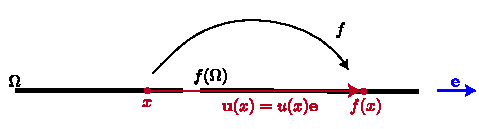
\includegraphics[scale=1.3]{figure/cinematica/spost1d}
\end{center}

Ovviamente, in questo contesto elementare, i punti possono solo spostarsi in direzione $\eb$, con intensità e verso specificati dal campo $u(x)$.
Il  gradiente dello spostamento è allora
\begin{definition}
\begin{equation}
	\Eb(x)=E(x) \eb\otimes \eb\coloneqq u'(x)\eb\otimes \eb=\big(f'(x)-1\big)\eb\otimes \eb.
\end{equation}
\end{definition}


La quantità \textit{adimensionale} $\Eb(x)$ definisce una \textit{misura locale di deformazione}. Se si immagina assegnata, l'equazione
%
\begin{equation}
	u'(x)=E(x)
\end{equation}
%
costituisce l'\textit{equazione di congruenza} che, corredata con opportune condizioni al contorno, determina il cosiddetto \textit{problema cinematico}.



\begin{exercise}
	Si consideri un segmento i cui estremi  $A$ e $B$ sono individuati da piazzamento $x(A)=0$ e $x(B)=L$. Si immagini che il punto $A$ sia fisso e che il segmento sia soggetto alla deformazione $E(x)=x/L+1$. Determinare il campo di spostamento.
\begin{svolgimento}
 Per determinare lo spostamento di tutti i punti occorre risolvere il problema 
	\begin{equation}
\begin{cases}
u'(x)=\dfrac{x}{L}+1 \qquad 0<x<L\\
u(0)=0.
\end{cases}
	\end{equation}
È immediato verificare che l'unica soluzione del problema è
\begin{equation}
	u(x)=x\left( 1+\frac{x}{2L} \right).
\end{equation} 	
L'estremo $B$ si sposta dunque della quantità $u(L)=3/2 L$ e si piazza in $f(L/2)=u(L)+L=5/2L$.
\end{svolgimento}
\end{exercise}	

Utilizzando la relazione tra spostamento e deformazione \eqref{spdef} è facile comprendere quale sia l'interpretazione fisica dell'assunzione $F(x)=f'(x)>0$. Sia $L$ la lunghezza del dominio $\Omega$, i cui estremi indichiamo con i punti $A$ e $B$; l'ipotesi che la deformazione sia monot\`{o}na crescente si traduce nella richiesta
\begin{equation}
	u'(x)> -1,
\end{equation}
che, integrata su $\Omega$, fornisce la condizione
\begin{equation}
	u(L)>u(0)-L.
\end{equation}
Se questa disuguaglianza non fosse soddisfatta, dopo la deformazione il punto $B$  potrebbe trovarsi a sinistra del punto $A$; in altri termini, il segmento orientato $\big( x(B)-x(A) \big)\eb$ che nella configurazione indeformata puntava da $A$  a $B$, secondo la direzione $\eb$, si potrebbe deformare in un segmento orientato secondo la direzione opposta, provocando interpenetrazione della materia. 

\begin{center}
	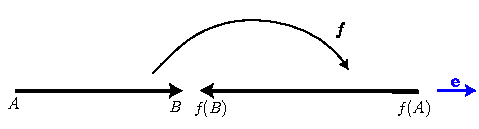
\includegraphics[scale=1.3]{figure/cinematica/orient1d}
\end{center}

Diciamo dunque che l'ipotesi $f'(x)>0$ serve a garantire la \textit{preservazione dell'orientazione dello spazio} (segmenti inizialmente orientati come $\eb$ rimangono così orientati) e che non vi sia \textit{interpenetrazioni} di materia. Osserviamo infine che vale la disuguaglianza stretta: se infatti fosse $u(L)-u(0)=-L$ gli estremi del segmento collasserebbero in un punto, circostanza che vogliamo evitare.

\section{Deformazioni omogenee}
Una deformazione è detta \textit{omogenea} se ha gradiente costante, $f'(x)=\alpha>0$. La generica rappresentazione di una deformazione omogenea è allora
\begin{definition}
\begin{equation}
f(x)=\alpha x+t \qquad t\in \Ro,
\end{equation}
\end{definition}
e dunque il corrispondente campo di spostamento risulta
\begin{equation}\label{spom}
	u(x)=f(x)-x=x(\alpha-1)+t.
\end{equation}

Una deformazione omogenea si definisce \textit{rigida} se lascia inalterate le distanze tra due punti:
\begin{equation}\label{fxfz}
|f(x)-f(z)|=|x-z| \qquad \forall x,z\in\Omega.
\end{equation}
Mostriamo adesso che una deformazione è rigida se e solo se il corrispondente campo di spostamento è  una \textit{traslazione} d'assieme:
\begin{equation}
u(x)=t \qquad t\in\Ro.
\end{equation}
Da \eqref{fxfz} segue che
\begin{equation}
\big(f(x)-f(z)\big)^2=\big(x-z\big)^2 \qquad \forall x,z\in\Omega;
\end{equation}
derivando rispetto a $x$ si ottiene 
\begin{equation}
2\big(f(x)-f(z)  \big)\,f'(x)=2(x-z) \qquad \forall x,z\in\Omega;
\end{equation}
e, derivando ancora rispetto a $z$, si conclude che
\begin{equation}
-2f'(x)f'(z)=-2 \qquad \forall x,z\in\Omega.
\end{equation}
Poiché quest'uguaglianza vale per ogni $x$ e $z$, deve necessariamente essere
\begin{equation}
\big( f'(x) \big)^2=1, \qquad \forall  x\in\Omega.
\end{equation}
Poiché si è assunto $f'(x)>0$, allora $f'(x)=1$ e dunque
\begin{equation}
	f(x)=x+t=:f_{\rm rig}(x), 
\end{equation}
dove $t$ è una costante arbitraria. Il corrispondente campo di spostamento è allora
\begin{equation}
u(x)=f(x)-x=t=:u_{\rm rig}.
\end{equation}
Tutti i punti si spostano della quantità $t$, che rappresenta dunque una traslazione rigida d'insieme.

La dimostrazione che se la deformazione è rigida allora preserva le lunghezze è banale e lasciata al lettore.

Osserviamo  che il campo di spostamento omogeneo \eqref{spom} può essere formalmente decomposto in due parti:
\begin{equation}
u(x)=u_{\rm def}(x)+u_{\rm rig}, \qquad  u_{\rm def}(x)\coloneqq u(x)-u_{\rm rig},
\end{equation}
in cui si è indicato con $u_{\rm rig}$ la componente rigida (costante) dello spostamento, mentre con $u_{\rm def}$ la componente deformativa, responsabile delle variazioni di lunghezza.

La nozione di deformazione rigida può essere utilizzata per selezionare delle buone \textit{misure di deformazione}, richiedendo che queste siano nulle in corrispondenza di deformazioni rigide. In particolare osserviamo che
\begin{equation}
 f_{\rm rig}'(x)=1, \quad C_{\rm rig}(x)=\big( f_{\rm rig}'(x)\big)=1, \qquad D_{\rm rig}(x)=\frac{1}{2}( C_{\rm rig}(x)-1)=0.
\end{equation}
Dunque il gradiente di deformazione e il campo scalare di Cauchy-Green non sono buone misure di deformazione, mentre il campo scalare di Green--Saint-Venant lo è, così come $E(x)$, visto che $E_{\rm rig}=F_{\rm rig}-1=0$.

\section{Teoria infinitesima}
In molte  applicazioni ha senso dunque limitarsi ad una teoria che consideri piccole deformazioni; vediamo adesso che forma questa ipotesi assume nel contesto elementare monodimensionale che stiamo qui considerando.

Abbiamo osservato che se una deformazione è rigida, il gradiente dello spostamento è $F_{\rm rig}=1$; possiamo allora pensare di considerare `piccola' una deformazione che si discosti di poco da quella rigida. Introduciamo dunque un parametro di piccolezza $\varepsilon$, definito come la più grande deformazione che può subire il corpo:
\begin{equation}
\varepsilon\coloneqq \sup_{x\in\Omega}|f'(x)-1|=\sup_{x\in\Omega}|E(x)|.
\end{equation}

La teoria dell’\textit{elasticità infinitesima} è quella  che si ottiene trascurando gli infinitesimi di ordine superiore al primo di $\varepsilon$. Ponendo $\varepsilon(x)\coloneqq |E(x)|$, poiché senz'altro $\varepsilon(x)\leq \varepsilon$, è possibile allora trascurare i termini dell'ordine di $\varepsilon^2(x)$.

Facendo questa ipotesi si ottiene che
\begin{equation}
C(x)=\big(f'(x)\big)^2=(E(x)+1)^2=1+2 E(x)+o\big(\varepsilon(x)\big)^2\simeq 1+2 E(x).
\end{equation}
Allora la misura di deformazione di Green--Saint-Venant diventa
\begin{equation}
D(x)=\frac12 \big( C(x)-1 \big)\simeq E(x).
\end{equation}
In teoria infinitesima allora quelle che avevamo stabilito essere buone misure di deformazione $D(x)$
 e $E(x)$ coincidono.






